% Options for packages loaded elsewhere
\PassOptionsToPackage{unicode}{hyperref}
\PassOptionsToPackage{hyphens}{url}
\documentclass[
  english,
  man]{apa6}
\usepackage{xcolor}
\usepackage{amsmath,amssymb}
\setcounter{secnumdepth}{-\maxdimen} % remove section numbering
\usepackage{iftex}
\ifPDFTeX
  \usepackage[T1]{fontenc}
  \usepackage[utf8]{inputenc}
  \usepackage{textcomp} % provide euro and other symbols
\else % if luatex or xetex
  \usepackage{unicode-math} % this also loads fontspec
  \defaultfontfeatures{Scale=MatchLowercase}
  \defaultfontfeatures[\rmfamily]{Ligatures=TeX,Scale=1}
\fi
\usepackage{lmodern}
\ifPDFTeX\else
  % xetex/luatex font selection
\fi
% Use upquote if available, for straight quotes in verbatim environments
\IfFileExists{upquote.sty}{\usepackage{upquote}}{}
\IfFileExists{microtype.sty}{% use microtype if available
  \usepackage[]{microtype}
  \UseMicrotypeSet[protrusion]{basicmath} % disable protrusion for tt fonts
}{}
\makeatletter
\@ifundefined{KOMAClassName}{% if non-KOMA class
  \IfFileExists{parskip.sty}{%
    \usepackage{parskip}
  }{% else
    \setlength{\parindent}{0pt}
    \setlength{\parskip}{6pt plus 2pt minus 1pt}}
}{% if KOMA class
  \KOMAoptions{parskip=half}}
\makeatother
% Make \paragraph and \subparagraph free-standing
\makeatletter
\ifx\paragraph\undefined\else
  \let\oldparagraph\paragraph
  \renewcommand{\paragraph}{
    \@ifstar
      \xxxParagraphStar
      \xxxParagraphNoStar
  }
  \newcommand{\xxxParagraphStar}[1]{\oldparagraph*{#1}\mbox{}}
  \newcommand{\xxxParagraphNoStar}[1]{\oldparagraph{#1}\mbox{}}
\fi
\ifx\subparagraph\undefined\else
  \let\oldsubparagraph\subparagraph
  \renewcommand{\subparagraph}{
    \@ifstar
      \xxxSubParagraphStar
      \xxxSubParagraphNoStar
  }
  \newcommand{\xxxSubParagraphStar}[1]{\oldsubparagraph*{#1}\mbox{}}
  \newcommand{\xxxSubParagraphNoStar}[1]{\oldsubparagraph{#1}\mbox{}}
\fi
\makeatother
\usepackage{graphicx}
\makeatletter
\newsavebox\pandoc@box
\newcommand*\pandocbounded[1]{% scales image to fit in text height/width
  \sbox\pandoc@box{#1}%
  \Gscale@div\@tempa{\textheight}{\dimexpr\ht\pandoc@box+\dp\pandoc@box\relax}%
  \Gscale@div\@tempb{\linewidth}{\wd\pandoc@box}%
  \ifdim\@tempb\p@<\@tempa\p@\let\@tempa\@tempb\fi% select the smaller of both
  \ifdim\@tempa\p@<\p@\scalebox{\@tempa}{\usebox\pandoc@box}%
  \else\usebox{\pandoc@box}%
  \fi%
}
% Set default figure placement to htbp
\def\fps@figure{htbp}
\makeatother
\ifLuaTeX
\usepackage[bidi=basic]{babel}
\else
\usepackage[bidi=default]{babel}
\fi
% get rid of language-specific shorthands (see #6817):
\let\LanguageShortHands\languageshorthands
\def\languageshorthands#1{}
\ifLuaTeX
  \usepackage[english]{selnolig} % disable illegal ligatures
\fi
\setlength{\emergencystretch}{3em} % prevent overfull lines
\providecommand{\tightlist}{%
  \setlength{\itemsep}{0pt}\setlength{\parskip}{0pt}}
% Manuscript styling
\usepackage{upgreek}
\captionsetup{font=singlespacing,justification=justified}

% Table formatting
\usepackage{longtable}
\usepackage{lscape}
% \usepackage[counterclockwise]{rotating}   % Landscape page setup for large tables
\usepackage{multirow}		% Table styling
\usepackage{tabularx}		% Control Column width
\usepackage[flushleft]{threeparttable}	% Allows for three part tables with a specified notes section
\usepackage{threeparttablex}            % Lets threeparttable work with longtable

% Create new environments so endfloat can handle them
% \newenvironment{ltable}
%   {\begin{landscape}\centering\begin{threeparttable}}
%   {\end{threeparttable}\end{landscape}}
\newenvironment{lltable}{\begin{landscape}\centering\begin{ThreePartTable}}{\end{ThreePartTable}\end{landscape}}

% Enables adjusting longtable caption width to table width
% Solution found at http://golatex.de/longtable-mit-caption-so-breit-wie-die-tabelle-t15767.html
\makeatletter
\newcommand\LastLTentrywidth{1em}
\newlength\longtablewidth
\setlength{\longtablewidth}{1in}
\newcommand{\getlongtablewidth}{\begingroup \ifcsname LT@\roman{LT@tables}\endcsname \global\longtablewidth=0pt \renewcommand{\LT@entry}[2]{\global\advance\longtablewidth by ##2\relax\gdef\LastLTentrywidth{##2}}\@nameuse{LT@\roman{LT@tables}} \fi \endgroup}

% \setlength{\parindent}{0.5in}
% \setlength{\parskip}{0pt plus 0pt minus 0pt}

% Overwrite redefinition of paragraph and subparagraph by the default LaTeX template
% See https://github.com/crsh/papaja/issues/292
\makeatletter
\renewcommand{\paragraph}{\@startsection{paragraph}{4}{\parindent}%
  {0\baselineskip \@plus 0.2ex \@minus 0.2ex}%
  {-1em}%
  {\normalfont\normalsize\bfseries\itshape\typesectitle}}

\renewcommand{\subparagraph}[1]{\@startsection{subparagraph}{5}{1em}%
  {0\baselineskip \@plus 0.2ex \@minus 0.2ex}%
  {-\z@\relax}%
  {\normalfont\normalsize\itshape\hspace{\parindent}{#1}\textit{\addperi}}{\relax}}
\makeatother

\makeatletter
\usepackage{etoolbox}
\patchcmd{\maketitle}
  {\section{\normalfont\normalsize\abstractname}}
  {\section*{\normalfont\normalsize\abstractname}}
  {}{\typeout{Failed to patch abstract.}}
\patchcmd{\maketitle}
  {\section{\protect\normalfont{\@title}}}
  {\section*{\protect\normalfont{\@title}}}
  {}{\typeout{Failed to patch title.}}
\makeatother

\usepackage{xpatch}
\makeatletter
\xapptocmd\appendix
  {\xapptocmd\section
    {\addcontentsline{toc}{section}{\appendixname\ifoneappendix\else~\theappendix\fi: #1}}
    {}{\InnerPatchFailed}%
  }
{}{\PatchFailed}
\makeatother
\keywords{keywords\newline\indent Word count: X}
\DeclareDelayedFloatFlavor{ThreePartTable}{table}
\DeclareDelayedFloatFlavor{lltable}{table}
\DeclareDelayedFloatFlavor*{longtable}{table}
\makeatletter
\renewcommand{\efloat@iwrite}[1]{\immediate\expandafter\protected@write\csname efloat@post#1\endcsname{}}
\makeatother
\usepackage{lineno}

\linenumbers
\usepackage{csquotes}
\usepackage{bookmark}
\IfFileExists{xurl.sty}{\usepackage{xurl}}{} % add URL line breaks if available
\urlstyle{same}
\hypersetup{
  pdftitle={PSY 8960-003 Reproducibility Project: Examining the Association Between Neuroticism and Loneliness Among College Students},
  pdfauthor={Caroline Armstrong1},
  pdflang={en-EN},
  pdfkeywords={keywords},
  hidelinks,
  pdfcreator={LaTeX via pandoc}}

\title{PSY 8960-003 Reproducibility Project: Examining the Association Between Neuroticism and Loneliness Among College Students}
\author{Caroline Armstrong\textsuperscript{1}}
\date{}


\shorttitle{Reproducibility Project}

\authornote{

The authors made the following contributions. Caroline Armstrong: Conceptualization, Writing - Original Draft Preparation, Writing - Review \& Editing.

Correspondence concerning this article should be addressed to Caroline Armstrong, 75 East River Parkway, Minneapolis, MN 55455. E-mail: \href{mailto:carolinearmstrong19@gmail.com}{\nolinkurl{carolinearmstrong19@gmail.com}}

}

\affiliation{\vspace{0.5cm}\textsuperscript{1} Department of Psychology, University of Minnesota}

\abstract{%
One or two sentences providing a \textbf{basic introduction} to the field, comprehensible to a scientist in any discipline.
Two to three sentences of \textbf{more detailed background}, comprehensible to scientists in related disciplines.
One sentence clearly stating the \textbf{general problem} being addressed by this particular study.
One sentence summarizing the main result (with the words ``\textbf{here we show}'' or their equivalent).
Two or three sentences explaining what the \textbf{main result} reveals in direct comparison to what was thought to be the case previously, or how the main result adds to previous knowledge.
One or two sentences to put the results into a more \textbf{general context}.
Two or three sentences to provide a \textbf{broader perspective}, readily comprehensible to a scientist in any discipline.
}



\begin{document}
\maketitle

{[}Insert intro here - 500 words{]}

\section{Methods}\label{methods}

\subsection{Participants}\label{participants}

Participants will be 400 university students enrolled in a Psychology course who opt to participate in a brief online survey for course credit.

\subsection{Measures}\label{measures}

\subsubsection{Demographics}\label{demographics}

Participants will be asked to indicate their age, gender, and racial and ethnic background. The exact questions and further details are shown in Appendix A.

\subsubsection{Big Five Inventory---Neuroticism Subscale}\label{big-five-inventoryneuroticism-subscale}

The Big Five Inventory---Neuroticism subscale (John et al., 1991) asks participants to indicate the extent to which they agree or disagree with eight statements about their personal characteristics or thinking and feeling tendencies in day-to-day life (e.g., ``I see myself as someone who is depressed, blue;'' ``I see myself as someone who worries a lot''). The response scale is an ordinal scale ranging from 1 = ``Disagree strongly'' to 5 = Agree strongly, with the intermediate response options being 2 = ``Disagree a little,''3 = ``Neutral; no opinion,'' and 4 = ``Agree a little.'' The complete scale instructions and items are shown in Appendix B.

A composite score is computed by summing the eight items.

\subsubsection{Loneliness in Context Questionnaire for College Students}\label{loneliness-in-context-questionnaire-for-college-students}

The Loneliness in Context Questionnaire for College Students (Asher \& Weeks, 2012) asks participants to indicate the frequency with which they feel lonely in various daily or weekly contexts typical for college students. Ten items tap different contexts (e.g., ``Class is a lonely place for me;'' ``I feel sad and alone at social events''), and participants respond on an ordinal scale ranging from 1 = ``Never'' to 5 = ``Always,'' with the intermediate response options being 2 = ``Hardly ever,'' 3 = ``Sometimes,'' and 4 = ``Most of the time.''

A composite score is computed by taking the average of the ten items.

\subsection{Procedure}\label{procedure}

The online survey will be developed and administered via Qualtrics. Potential participants will be informed about the study via online communications from the university's Psychology Department and may choose to complete the study from their personal device at any time during the current academic semester.

Participants will provide informed consent by indicating that they would like to proceed to the survey questions after reading a brief written explanation (on the first page of the Qualtrics survey) describing what they will be asked to do (i.e., complete an approximately five-minute survey asking them about their personality and mental state) and the possible risks (i.e., experiencing various forms of psychological discomfort while reflecting on oneself and one's feelings) and benefits (i.e., possible improvements in scientific knowledge) of their participation.

Of note, the consent will include a clause indicating that participants' de-identified data (i.e., their responses to all survey questions, including demographic information, but NOT including any information such as IP addresses that could be used to identify them) may be used by other researchers for any purpose and shared on an online, publicly available platform.

Participants who affirm their consent will proceed to the survey questions. All participants will complete the Demographic questions first. To control for possible order effects, participants will be randomized to complete either the Big Five Inventory---Neuroticism subscale or the Loneliness in Context Survey second. The third section will consist of whichever measure participants did not complete second.

Following the survey questions, participants will view a short debriefing description indicating the study aim and providing information about campus mental health resources that may be of aid if participants found that reflecting on their mental state and day-to-day loneliness caused distress or prompted them to think about seeking psychological help.

\subsection{Data analysis}\label{data-analysis}

Descriptive statistics will be computed for demographic variables, including mean and standard deviation for age and, for gender and racial and ethnic identities endorsed, counts and proportions.

I will compute Pearson's \emph{r} for the association between the composite neuroticism and loneliness scores and test the hypothesis that this correlation is significantly (\(\alpha\) = .001) greater than \emph{r} = .00 in this sample.

My choice to calculate Pearson's \emph{r} (e.g., versus Spearman's \emph{r}) is based on the fact that the distributions of simulated data for \texttt{neuroticism} and \texttt{loneliness} are both approximately normal, an assumption of Pearson's \emph{r} (see below for relevant computations and visualizations).

\pandocbounded{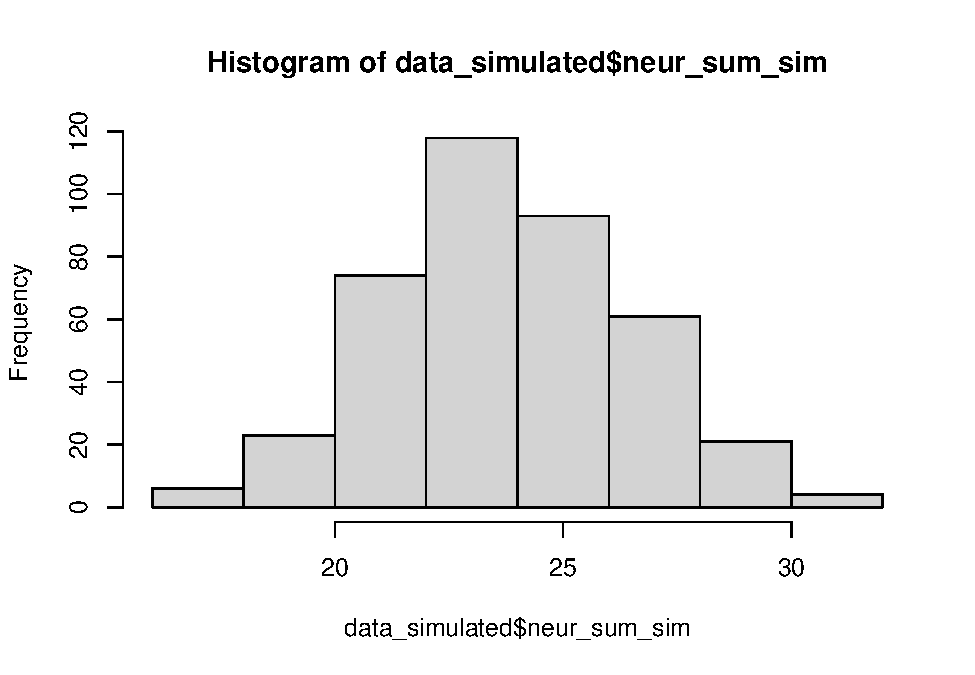
\includegraphics[keepaspectratio]{reproducibility-project-manuscript_files/figure-latex/histogram-1.pdf}} \pandocbounded{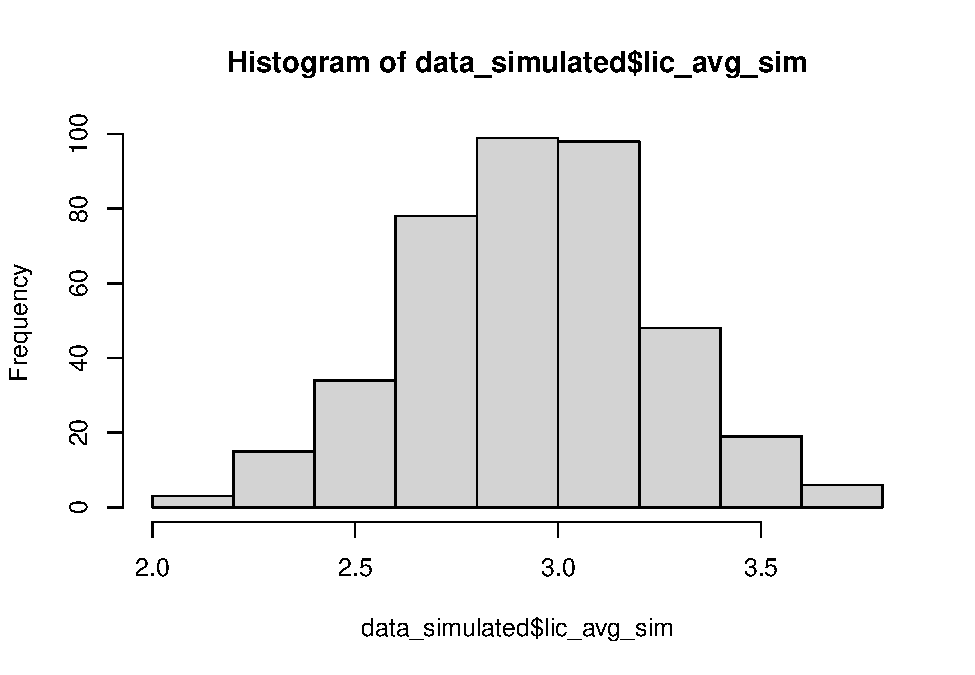
\includegraphics[keepaspectratio]{reproducibility-project-manuscript_files/figure-latex/histogram-2.pdf}}

\section{Results}\label{results}

Using my simulated data,

Descriptive statistics will be computed for demographic variables, including mean and standard deviation for age and, for gender and racial and ethnic identities endorsed, counts and proportions.

\begin{verbatim}
##   mean(age_sim) SD(age_sim)
## 1        19.795    1.287291
\end{verbatim}

\begin{verbatim}
## # A tibble: 3 x 3
##   gender_sim                   n   freq
##   <chr>                    <int>  <dbl>
## 1 Man                        121 0.302 
## 2 Nonbinary or genderqueer    13 0.0325
## 3 Woman                      266 0.665
\end{verbatim}

\begin{verbatim}
## # A tibble: 7 x 3
##   race_ethn_sim                           n   freq
##   <chr>                               <int>  <dbl>
## 1 American Indian or Alaska Native        3 0.0075
## 2 Asian                                  41 0.102 
## 3 Black or African American              48 0.12  
## 4 Hispanic or Latino                     55 0.138 
## 5 Middle Eastern or North African        21 0.0525
## 6 Native Hawaiian or Pacific Islander     6 0.015 
## 7 White                                 226 0.565
\end{verbatim}

\begin{verbatim}
## 
##  Pearson's product-moment correlation
## 
## data:  data_simulated$neur_sum_sim and data_simulated$lic_avg_sim
## t = -1.8885, df = 398, p-value = 0.9702
## alternative hypothesis: true correlation is greater than 0
## 95 percent confidence interval:
##  -0.1752443  1.0000000
## sample estimates:
##         cor 
## -0.09423871
\end{verbatim}

\pandocbounded{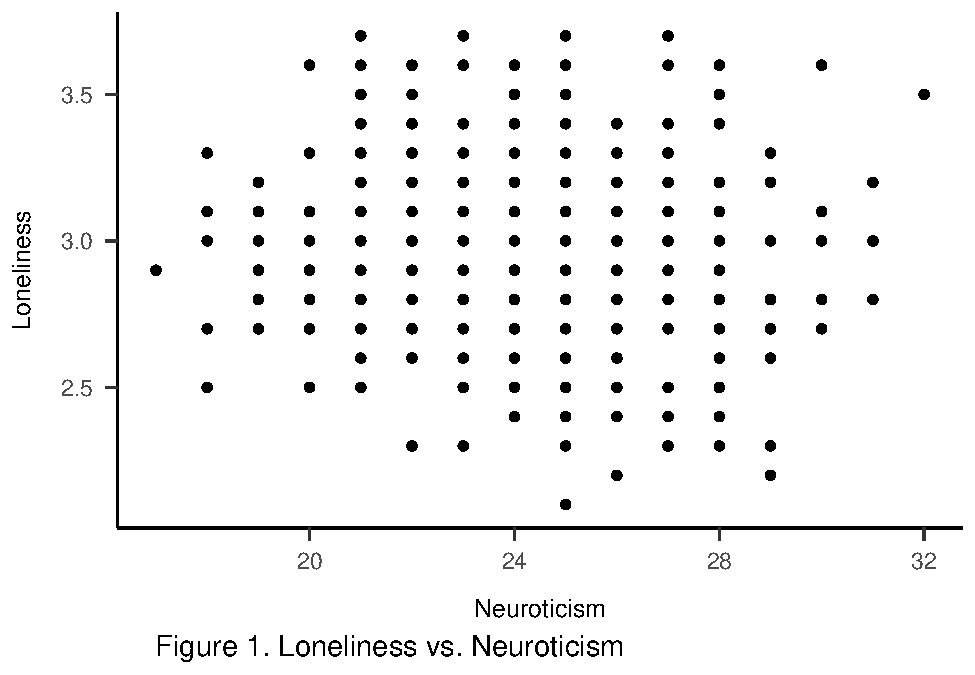
\includegraphics[keepaspectratio]{reproducibility-project-manuscript_files/figure-latex/unnamed-chunk-5-1.pdf}}

\newpage

\section{References}\label{references}

\phantomsection\label{refs}

\section{Appendix A}\label{appendix-a}

\subsection{Demographics}\label{demographics-1}

Participants will be asked the following demographic questions:

What is your current age in years? \emph{(free text response with data validation to ensure that a two-digit integer is entered)}

How would you describe your gender? \emph{(three possible answer choices, of which one may be selected: (1) Man, (2) Woman, (3) Nonbinary or genderqueer)}

How would you describe your racial and ethnic background? Select all that apply. \emph{(seven possible answer choices, of which multiple may be selected: (1) American Indian or Alaska Native, (2) Asian, (3) Black or African American, (4) Hispanic or Latino, (5) Middle Eastern or North African, (6), Native Hawaiian or Pacific Islander, (7) White)}

\newpage

\section{Appendix B}\label{appendix-b}

\subsection{Big Five Inventory: Neuroticism Subscale (John et al., 1991)}\label{big-five-inventory-neuroticism-subscale-john-et-al.-1991}

Instructions: \emph{In this section, you will read a number of characteristics that may or may not apply to you. For example, do you agree that you are someone who is talkative? Consider how you think and feel in everyday life and indicate how much you agree or disagree with each statement. Remember that there are no right or wrong answers because people think and feel very differently from one another. Just read each question carefully and answer honestly.}

I see myself as someone who\ldots{}

Is depressed, blue
Is relaxed, handles stress well
Can be tense
Worries a lot
Is emotionally stable, not easily upset
Can be moody
Remains calm in tense situations
Gets nervous easily

\newpage

\section{Appendix C}\label{appendix-c}

\subsection{Loneliness in Context Questionnaire for College Students (Asher \& Weeks, 2012)}\label{loneliness-in-context-questionnaire-for-college-students-asher-weeks-2012}

Instructions: \emph{Sometimes people can feel lonely in their day-to-day lives. The items in this section ask about your feelings in different contexts. On the scale directly below/beside each item indicate how often you feel the way the item describes. There are no right or wrong answers because people can feel very differently from one another. Just describe how you feel in these contexts (1 = Never, 2 = Hardly Ever, 3 = Sometimes, 4 = Most of the Time, 5 = Always).}

Class is a lonely place for me.\\
I am lonely in the evening.
My place of residence is a lonely place for me.
My free time is a lonely time for me.
I feel sad and alone on weekends.
I am lonely with other people.
I feel sad and alone at social events.
I am lonely during meal times.
I feel sad and alone when I am studying.
Bedtime is a lonely time for me.

When you do feel lonely, how lonely do you feel? \emph{(0 = I never feel lonely, 1 = Slightly lonely, 2 = Somewhat lonely, 3 = Very lonely, 4 = Extremely lonely, 5 = Painfully lonely)}


\end{document}
